\section{Jet flavour tagging}
\label{sec:ch6_btag}

Jet flavour tagging is used to distinguish $b$-quark originating jets ($b$-jets) from other jet flavours.

$b$-jets are identified through displaced $b$-hadron decays, which have a lifetime of about $1.5$~ps. Therefore a boosted $b$-hadron can travel several millimetres before decaying.
The decay tracks therefore typically have large impact parameters and originate from a secondary vertex displaced from the PV.
Charm hadrons produced in the $b$-hadron decay can further decay at an additional displaced vertex.
These features are used for jet flavour tagging.

The tagger uses the GN2v01 algorithm, which is based on a transformer neural network trained on simulated events~\cite{ATLAS2026GN2}.
Its inputs include jet and track kinematics, track impact parameters, and hit variables.
These variables are first encoded as a numerical vector for each track.
Within the transformer, each vector is updated through self-attention, using information from the other tracks.
Correlations between tracks can thereby be used to recognise a common displaced origin without requiring explicitly reconstructed secondary vertices as separate inputs.
The network then calculates a weight for each track using its updated vector and adds the weighted vectors together, which is called attention pooling.

The resulting vector is used for the main task of jet-flavour classification.
It is also combined with the individual track vectors for two auxiliary tasks: identifying track origins and predicting whether pairs of tracks originate from the same vertex.
The three tasks share the transformer and are trained jointly, helping it learn the decay structure relevant to flavour tagging.
The network and its three tasks are illustrated in Figure~\ref{fig:ch6_gn2}.

The jet-flavour classifier produces four outputs for the $b$-jet, $c$-jet, hadronic-$\tau$ and light-jet hypotheses, where light jets originate from $u$, $d$ or $s$ quarks or gluons.
These outputs are combined into a single discriminant, $D_b$, which compares the $b$-jet output with a weighted combination of the other three outputs.
Larger values favour the $b$-jet hypothesis.
The GN2v01 85\% working point is used in this analysis, corresponding to a nominal $b$-jet tagging efficiency of 85\%.

\begin{figure}[htbp]
    \centering
    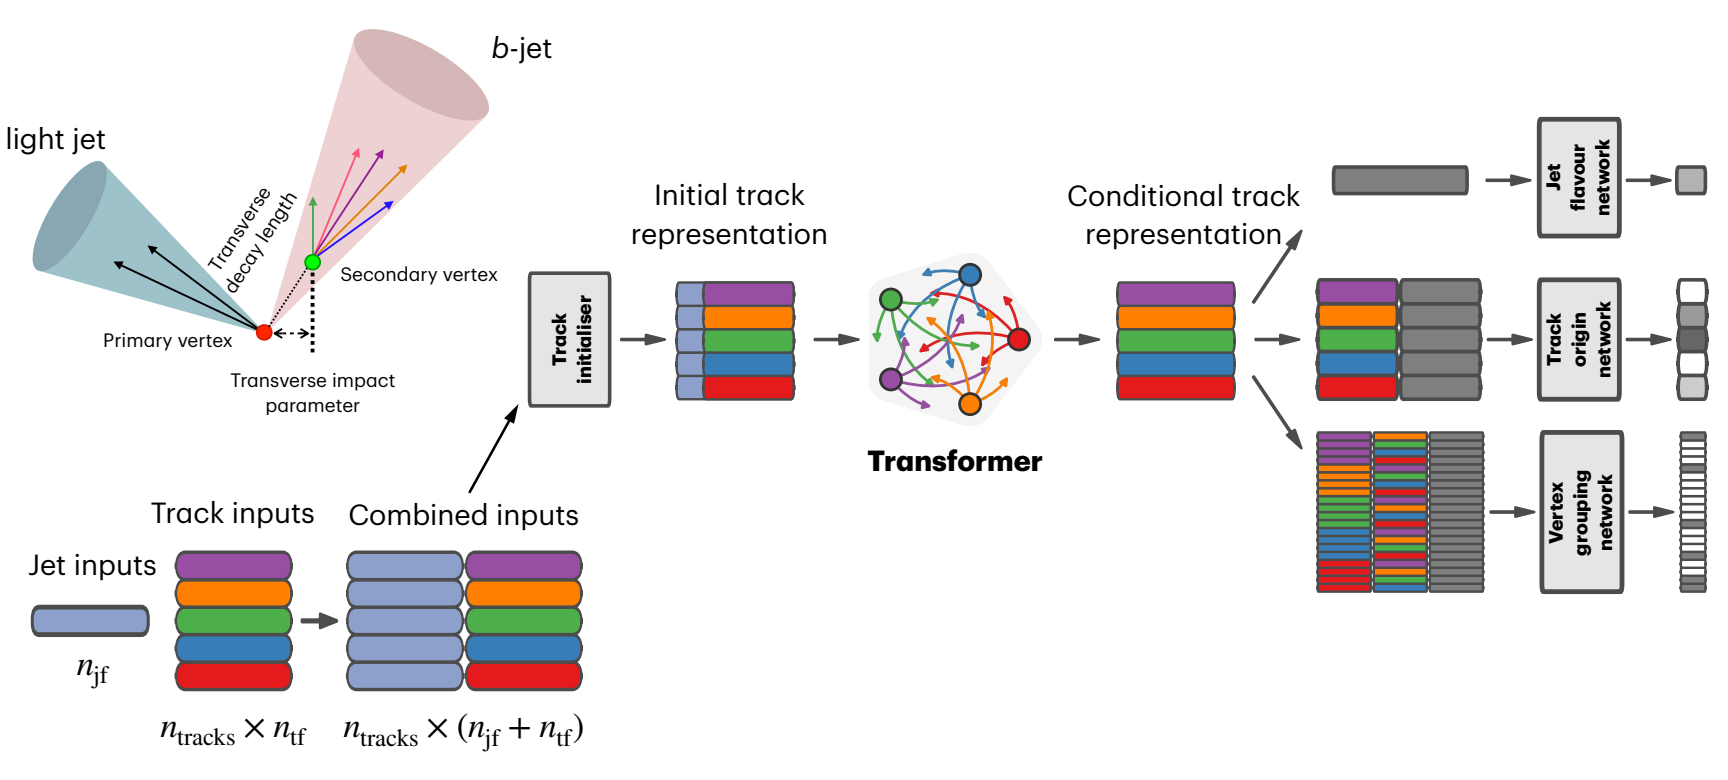
\includegraphics[width=\textwidth]{output/ch6/figures/gn2_architecture.png}
    \caption[GN2 flavour-tagging architecture]{GN2 flavour-tagging architecture. The jet variables are appended to the input vector of each track before processing by the track initialiser and transformer. The resulting track vectors and their weighted combination are passed to the jet-flavour, track-origin and vertex-grouping networks. The symbols $n_{\mathrm{jf}}$, $n_{\mathrm{tf}}$ and $n_{\mathrm{tracks}}$ denote the numbers of jet variables, track variables and tracks, respectively~\cite{ATLAS2026GN2}.}
    \label{fig:ch6_gn2}
\end{figure}

\subsection{Calibration}

The $b$-jet tagging efficiency and the $c$-jet and light-jet mistagging efficiencies are measured in flavour-enriched data samples and compared with simulation~\cite{ATLAS2026GN2}. % 详细写出是哪个sample测量哪个flacour tagging/mistagging efficiecny，不要用这种flavour-enrivhed抽象词概括。
A tagged jet of flavour $f$ is assigned a weight $\mathrm{SF}_f$.%不需要介绍SF的具体公式，把
Untagged jets also require a correction because the probability for a jet to fail the tag is $1-\epsilon_f$, where $\epsilon_f$ is the tagging efficiency for flavour $f$.
The weight for an untagged jet is therefore
\begin{align}
    w_f^{\mathrm{untagged}}
    =\frac{1-\epsilon_f^{\mathrm{data}}}{1-\epsilon_f^{\mathrm{MC}}}
    =\frac{1-\mathrm{SF}_f\epsilon_f^{\mathrm{MC}}}{1-\epsilon_f^{\mathrm{MC}}},
    \label{eq:ch6_btag_untagged}
\end{align}
where $\epsilon_f^{\mathrm{data}}$ and $\epsilon_f^{\mathrm{MC}}$ are the efficiencies in data and simulation, respectively.
The simulated event weight is multiplied by the product of the factors for its tagged and untagged jets.
Flavour-tagging corrections therefore affect both the zero-tag and tagged event categories.
